\glsresetall{} 
\chapter{Operations Concepts}

\lettrine[lines=2, findent=0pt, nindent=5pt]{B}{} efore discussing the
\gls{pops} it is necessary to go over basic terminology.  Without doing so, it
may become very easy for descriptions to become unclear or imprecise

\section{General Definitions}

\begin{description} 

    \item[Ephemeris] is a set of data that describes the position and velocity
	of a celestial object at specific times. They are used, in this
	context, to describe the positions and velocities of satellites.
	Typically, this information is stored as orbital state vectors. These
	state vectors have a position component, $\sev{r}$, a velocity
	component, $\sev{v}$, and an epoch for those vector, $e$. See section
	\ref{sgp4_section} for a more detailed discussion on ephemerides.

    \item[Area of Interest] An \gls{aoi} is a general concept for a region on
	the Earth that is of some particular importance to an operator. It is
	the region in which one or more spacecraft should observe through some
	means.  \glspl{aoi} can be specified as a point target, a polygon, or a
	latitude range. See section \ref{aoi_def} for an exhaustive definition
	in this context. 

    \item[Field of View] The \gls{fov} is the extent to which a sensor or
	instrument may observe the outside world at a given time. The size and
	shape of an \gls{fov} varies based on the design of the sensor or
	instrument in question. Unless otherwise specified, for the purposes of
	this thesis, it may be assumed that \glspl{fov} are conical.
	Specifically, the \gls{fov} is defined by a single half-angle,
	$\theta$. Suppose an instrument is pointing along some vector,
	$\sev{u}$. Let us define another vector, $\sev{v}$ such that the angle
	between it and $\sev{u}$ is $\theta$. The \gls{fov} is the volume
	described by rotating $\sev{u}$ around $\sev{v}$.


    \item[Field of Regard] The \gls{for} is similar to the \gls{fov}. Instead
	of being the area a sensor can observe in a singular time instant, the
	\gls{for} is the area a sensor can possibly observe by changing its
	orientation given some external constraint. It is not possible to
	observe the entire \gls{for}; Rather, only a subset of the \gls{for}
	can be observed. This subset is the instrument's \gls{fov}.  For
	example, let us consider an optical sensor fixed to a spacecraft
	orbiting the earth. The position of the sensor at particular time
	instant is given by the spacecraft's orbit and cannot be changed unless
	a propulsive manoeuvre is performed. Of course, the position of sensor
	can be changed slightly by changing the attitude of the spacecraft,
	since the instrument is most likely not located at the spacecraft's
	centre of mass. But, this can be ignored since the distance the
	instrument can translate is negligible compared to its orbit.
	Conversely, The orientation of the instrument can be changed, and this
	has a meaningful effect on the \gls{for}. If no constraints are put on
	the attitude of the spacecraft, the \gls{for} is everywhere, since the
	instrument can be pointed in any direction. This is not always true
	though so let us say the spacecraft can only point an angle, $\alpha$,
	off nadir.  The \gls{for} would then be the cone described by the
	half-angle $\alpha + \theta$, where $\theta$ is again the half-angle of
	the conical sensor.  See Figure \ref{fig:fovfor} for an illustration of
	this example.  The larger blue cone is the \gls{for}. The red cone is
	the sensor's actual \gls{fov}. Its boresight is offset from the blue
	cone's.


\begin{figure} 
    \centering
    \begin{minipage}[c]{0.45\textwidth}
	\centering
	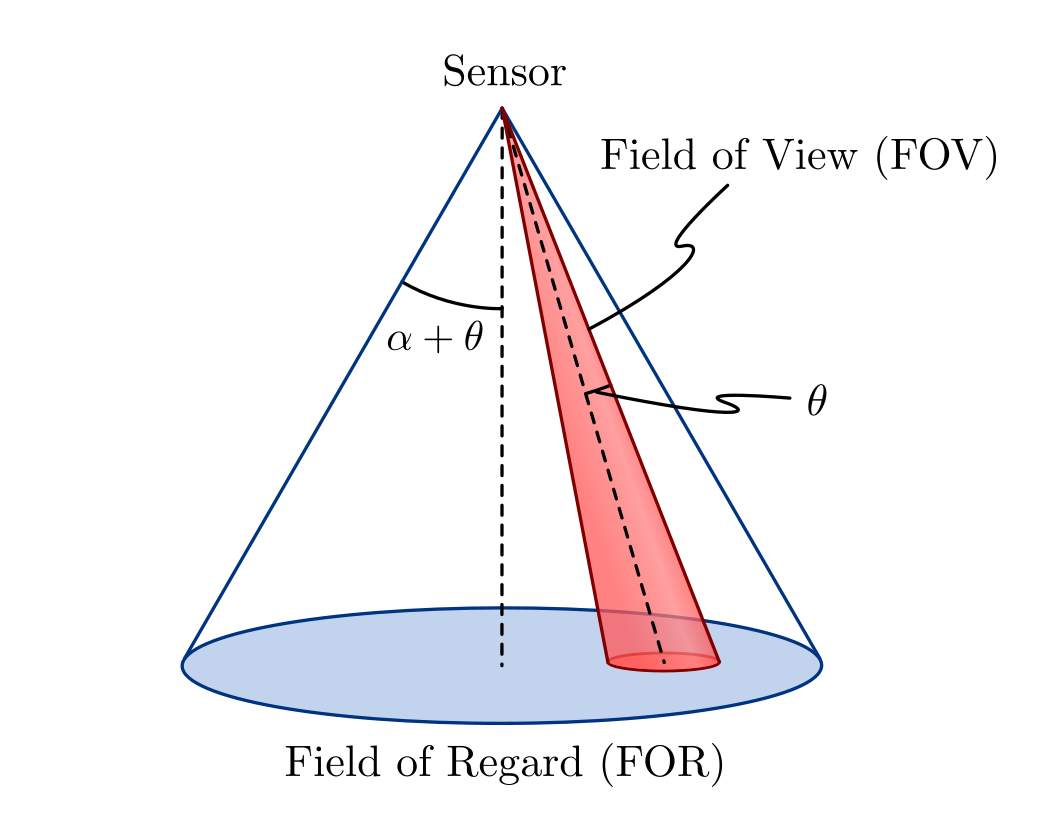
\includegraphics[width=\textwidth]{FOV_FOR.png} \caption{Illustration of conical 
	FOV(red) and FOR(blue)}
	\label{fig:fovfor} 
    \end{minipage}
    \hfill
    \begin{minipage}[c]{0.45\textwidth}
	\centering
	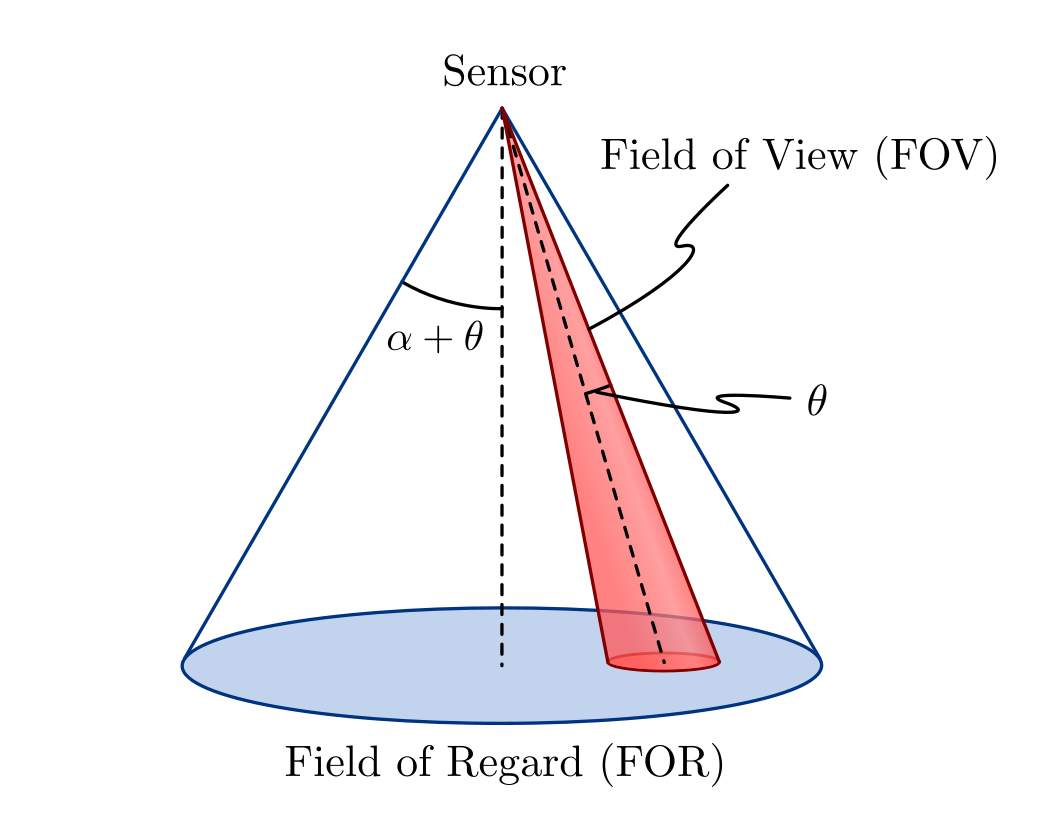
\includegraphics[width=\textwidth]{FOV_FOR.png} \caption{FOV(red),
	FOR(blue) Illustration}
	\label{fig:fovfor2} 
    \end{minipage} 
\end{figure}

    \item[Footprint] The footprint is the area on Earth that can be observed by
	an instrument's \gls{fov} or \gls{for} at a given time. It can be found
	by intersecting the \gls{fov} or \gls{for} with the surface of the
	Earth.  These intersection points form a boundary and the enclosed area
	within this boundary is the footprint. For clarity, it should be
	assumed that footprint refers to an \gls{for}'s footprint, unless
	otherwise specified.

    \item[Swath] If a sensor is moving over time, its footprint will move with
	it. A swath is the union of all footprints over a time range.  It is
	the region on Earth that can be possibly observed at some point by the
	sensor.

    \item[Horizon Swath] A horizon swath is a special case where the entire
	Earth is within the sensor's \gls{for}. This may be true for certain
	\gls{rf} payloads. In this case, the sensor can only `see' up until the
	horizon. That is, the `horizon' footprint is all of the points on Earth
	whose tangent line intersects with the sensor. Again, as the horizon
	footprint moves, this forms the horizon swath.

\end{description}



\section{Time Tag Commands}

At the \gls{sfl}, satellites are commanded through the use of the \gls{nsp}.
\gls{nsp} commands are a custom standard developed by \gls{sfl} to facilitate
ground and intra-satellite communication. They are designed to minimize the
effects of low-bandwidth radio communication links that are prone to error.
These commands handle all aspects of nominal operation, from turning individual
components on or off, to specifying attitude modes or initiating data
transfers. Once a command is sent, it is executed immediately upon being
received. This, of course, poses an obvious problem, how should a spacecraft be
commanded when it does not have a direct communication link with a ground
station. To address this, there exist \glspl{ttc}. These are \gls{nsp} commands
that have been prepended with a timestamp. When the spacecraft's internal clock
reaches the time specified in the timestamp, that command is exectuted. These
\glspl{ttc} are prepared in advance by an operator and uploaded in bulk to the
spacecraft. This allows operators to control the spacecraft when direct
communication cannot be established.



% This should be moved somewhere else
\section{Equator Crossing Algorithm}

For a given ephemeris, it is useful to determine each ``pass'' of that orbit.
That is, for each ephemeris point, an index should be assigned to it which
indicates how many times the spacecraft has orbited the Earth. In this way, if
we have some time range and we wish to see the next `pass,' we would simply
take that time range's pass index and add 1.

There are many ways a pass may be defined. For example we could specify a
latitude and longitude range and whenever the spacecraft is in this range, that
oculd be considered a singular pass.  Generally, though, epehemeris data is not
given in latitude or longitude, rather it is given in a cartesian position in
some \gls{eci} or \gls{ecef} reference frame.  So for each position in the
ephemeris, the position vector will need to be converted to latitude and
longitude. 

This is a completely acceptable approach but we may also simplify the problem.
Instead of taking a latitude and longitude range, we could instead increment
the pass index when the spacecraft crosses the equator and goes from the
southern to the northern hemisphere. This would be when the spacecraft's
position goes from a negative to a positive latitude. This definition of a pass
has a few advantages. That being, we only need to do one check to determine a
pass boundary. It also has the benefit of indexing the entire ephemeris. Still
for this method, we need to convert from cartesian postiion to at least
latitude.

Let us make one further simplification by assuming that the x-y plane of the
ephemeris's coordinate system is very near to the Earth's equitorial plane.
This is not true for all cooordinate systems but it is true for the ephemerides
used by \gls{pops}. By making this assumption, we no longer need to calculate
the latitude of the spacecraft; rather, we can instead only look at the
spacecraft's position along the z-axis. This is useful because the spacecraft's
$z$-position will oscillate between some positive and negative extrema, which
are determined by the orbit's inclination and excentricity. 

There is a complicating factor that should be accounted for, though. In time,
the spacecraft's position is periodic, but when considering only the
spacecraft's $z$-position in an ephemeris, there is no guarantee that there is
a contant timestep between position values. Additional data-points may be
injected for periods where greater accuracy is desired and vice-versa.  

% TODO: Add two figures, one showing a sinusoidal z-comp in time, and one
% showing one with additional data points added, making it oblong.

Now the problem becomes: for an array of z-p 

\newcommand*\Let[2]{\State #1 $\gets$ #2}

\begin{algorithm} 
    \caption{Negative-Positive Crossing Search Algorithm} 
    \begin{algorithmic}[1] 
	\Require{\se{z}is a $1\times N$ array } 

	\Function{FindAllCrossovers}{$s, f, \se{z}$}
	    \Let{$c$}{$0$}
	    \Let{$\se{p}$}{$\{  \}$}
	    \State $\se{p}.append( \mathrm{\Call}  )$
	    \While{}
	\EndFunction

	\State

	\Function{FindNextCrossover}{$i, s, f, \se{z}$} 
	\Let{$j$}{$i+s$}
	\If{$j > length(\se{z})$} 
	    \State $s = \mathrm{s \times f}$  
	\ElsIf{$j = length(\se{z})$}
	    \State \Return $-1$	  \Comment{Search has completed}
	\ElsIf{ $(\se{z}[i] < 0) \lor (\se{z}[j] > 0)$ }
	    \If{$s=1$}
	    \State \Return $i$ \Comment{Crossover index found}
	    \Else
		\State $s = ceil(s \times f)$
	    \EndIf
	\Else
	    \State $i=j$
	\EndIf
	\State \Return \Call{FindNextCrossover}{$i, s, f, \se{z}$}
	\EndFunction 
    \end{algorithmic} 
\end{algorithm}

\begin{algorithm} 
    \caption{Negative-Positive Crossing Search Algorithm} 
    \begin{algorithmic}[1] 
	\Require{$x$ and $y$ are packed strings of equal length $n$} 
	\Statex
	\Function{Distance}{$x, y$} 
	    \Let{$z$}{$x \oplus y$} \Comment{$\oplus$: bitwise exclusive-or} 
	    \Let{$\delta$}{$0$} 
	    \For{$i \gets 1 \textrm{ to } n$}
		\If{$z_i \neq 0$} 
		    \Let{$\delta$}{$\delta + 1$} 
		\EndIf 
	    \EndFor 
	    \State \Return{$\delta$} 
	    \State \Return{\Call{Distance}{$x, y$}}
	\EndFunction 
    \end{algorithmic} 
\end{algorithm}







